\begin{frame}
    \frametitle{Comparison of Prediction Methods}
\textbf{EG01-23 Constant Power Demand Transition Scenario}

\begin{figure}[htbp!]
    \begin{center}
      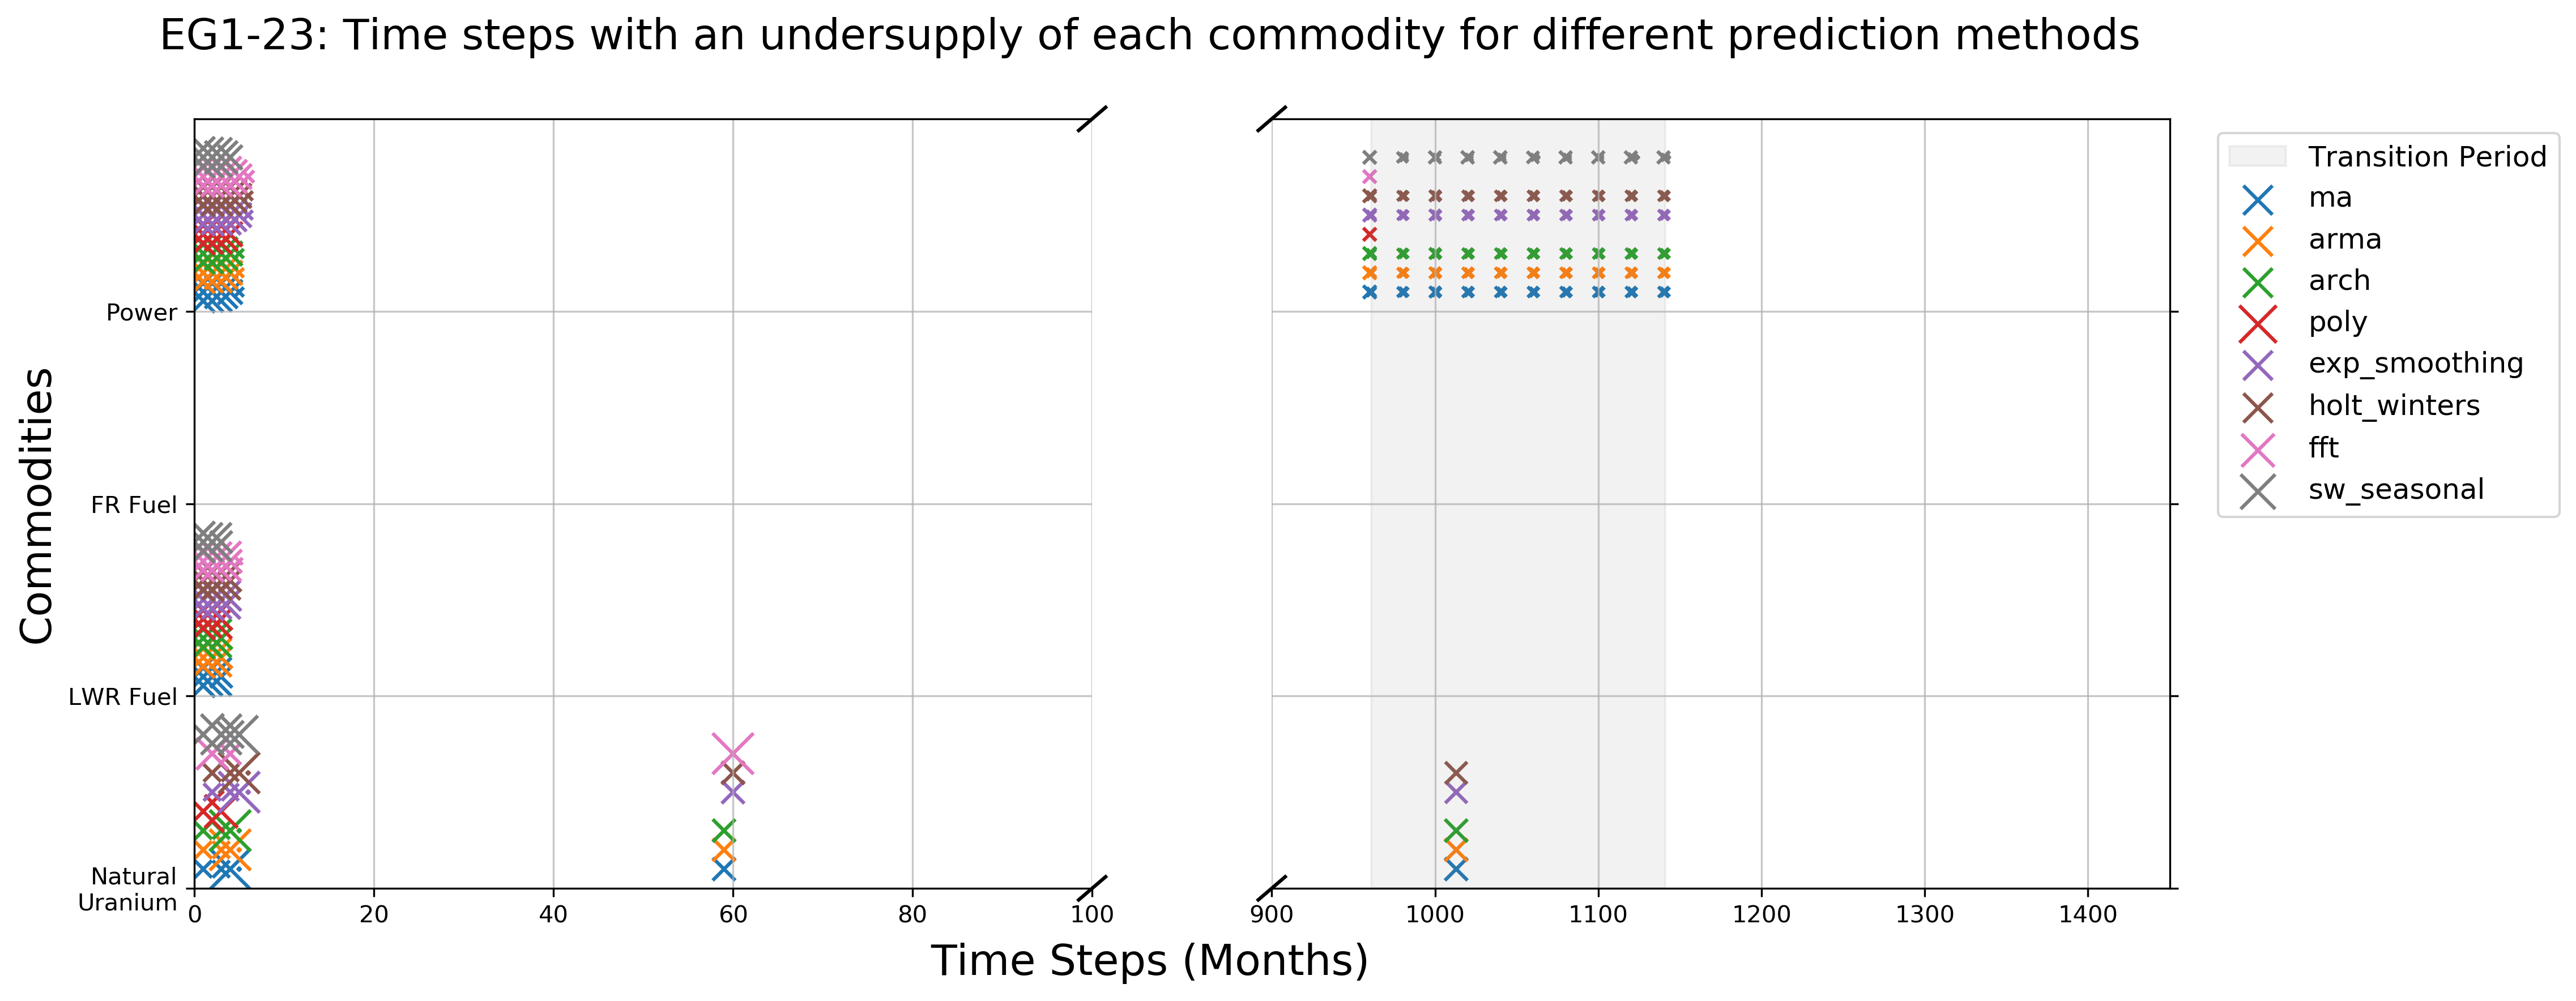
\includegraphics[width=\textwidth]{images/eg23-undersupply.png}
    \end{center}
          \caption{Time dependent undersupply of commodities for different
          prediction methods for the EG01-23 Transition Scenario with Constant Power Demand. The
          size of each cross is based on the size of the undersupply.
          Fewer crosses on plot indicates the method is more successful at preventing undersupply 
          of each commodity}
  \end{figure}
\end{frame}

\begin{frame}
    \frametitle{Comparison of Prediction Methods}
    \textbf{EG01-23 Constant Power Demand Transition Scenario}
\begin{figure}[htbp!]
    \begin{center}
      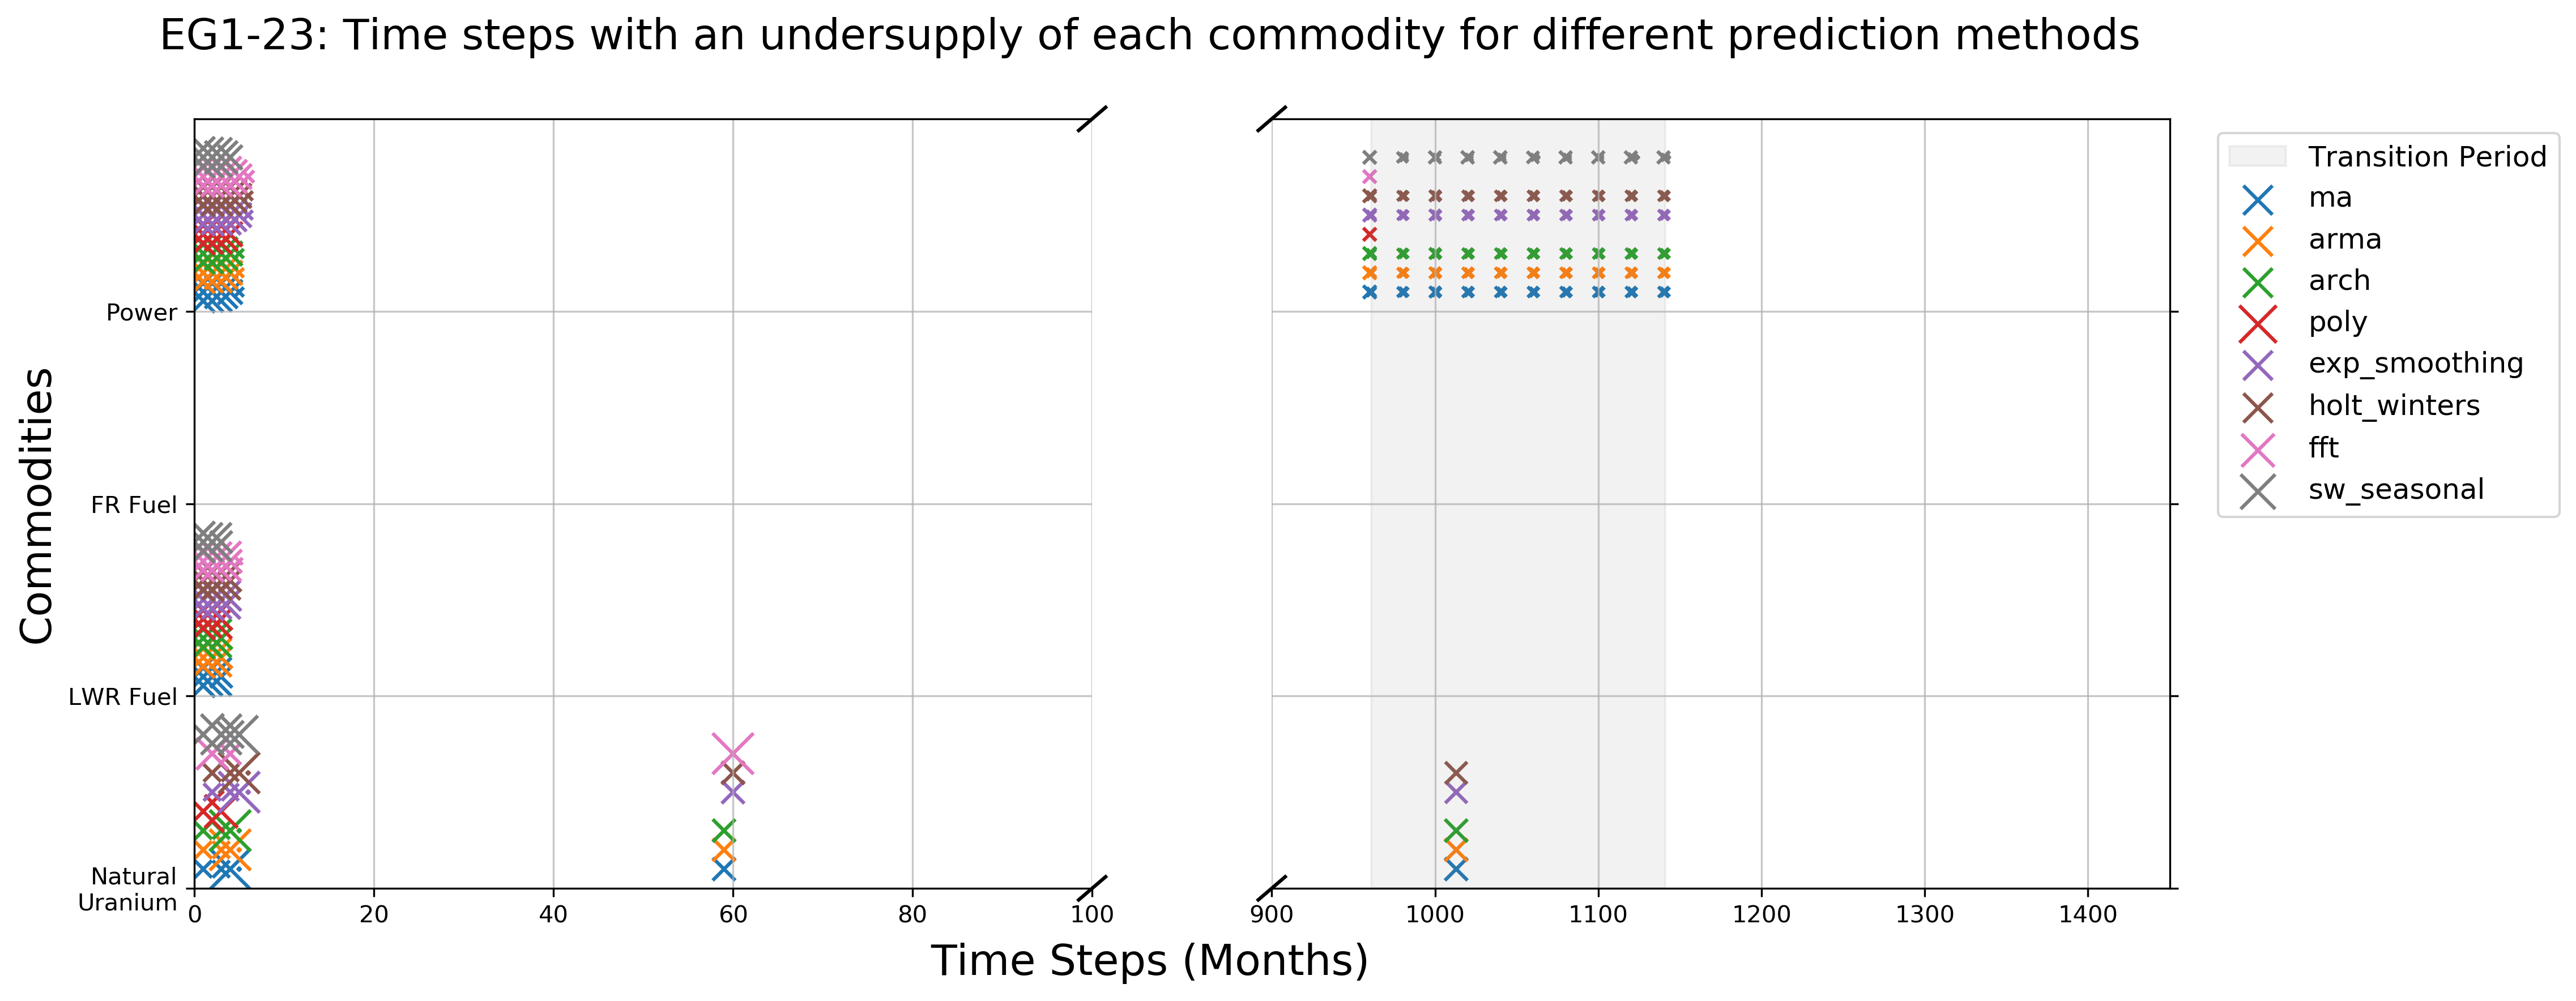
\includegraphics[width=\textwidth]{images/eg23-undersupply.png}
    \end{center}
          \caption{Time dependent undersupply of commodities for different
          prediction methods for the EG01-23 Transition Scenario with Constant Power Demand. The
          size of each cross is based on the size of the undersupply.
          Fewer crosses on plot indicates the method is more successful at preventing under capacity 
          of each commodity}
  \end{figure}
\end{frame}

\begin{frame}
    \frametitle{Comparison of Prediction Methods}
\textbf{EG01-24 Constant Power Demand Transition Scenario}
\begin{figure}[htbp!]
    \begin{center}
      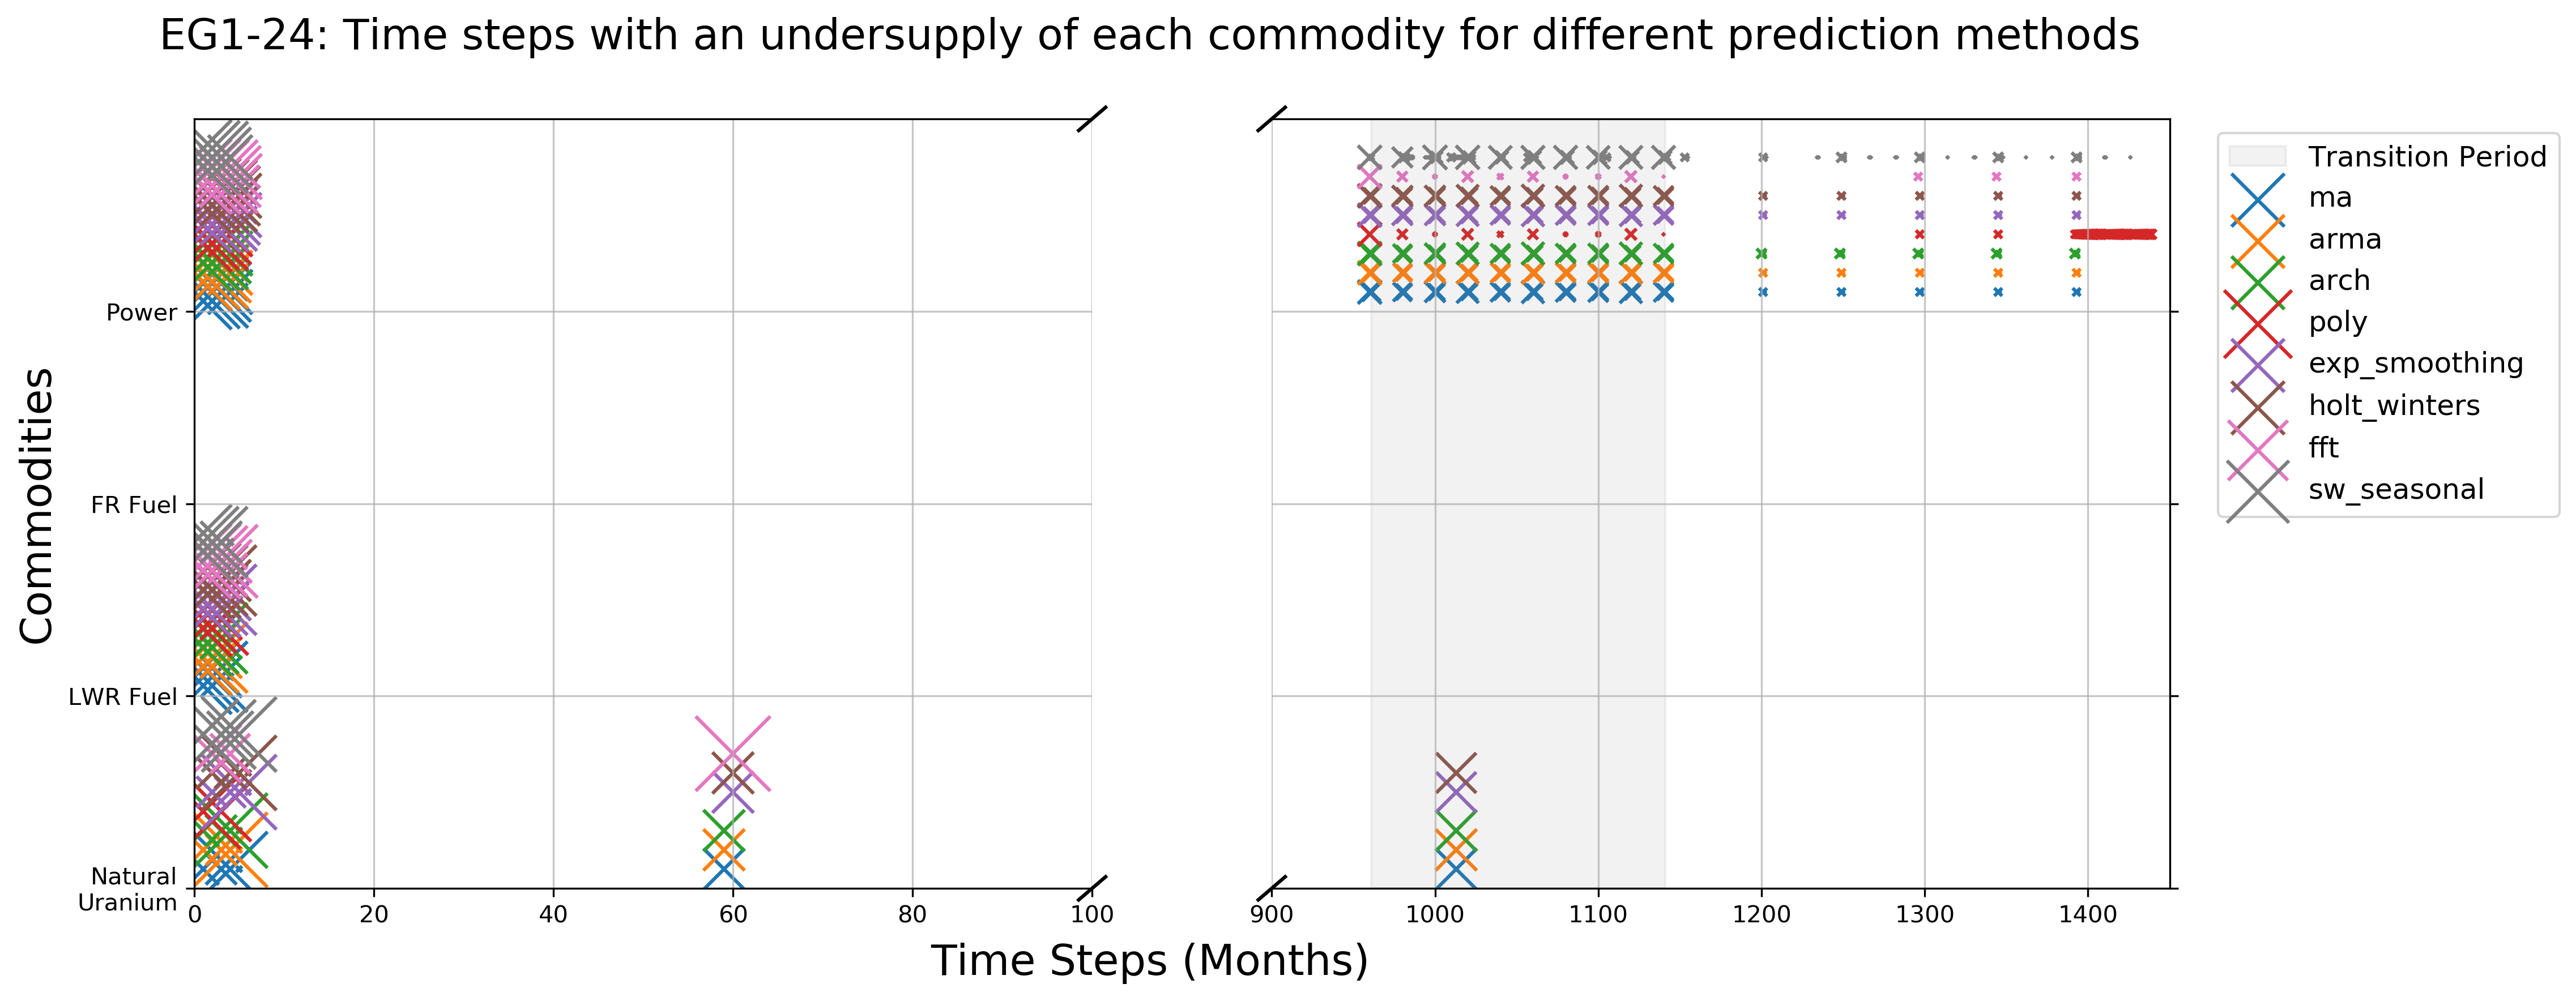
\includegraphics[width=\textwidth]{images/eg24-undersupply.png}
    \end{center}
          \caption{Time dependent undersupply of commodities for different
          prediction methods for the EG01-24 Transition Scenario with Linearly Increasing Power Demand.The
          size of each cross is based on the size of the undersupply.
          Fewer crosses on plot indicates the method is more successful at preventing undersupply 
          of each commodity}
  \end{figure}
\end{frame}

\begin{frame}
    \frametitle{Comparison of Prediction Methods}
    \textbf{EG01-24 Constant Power Demand Transition Scenario}
\begin{figure}[htbp!]
    \begin{center}
      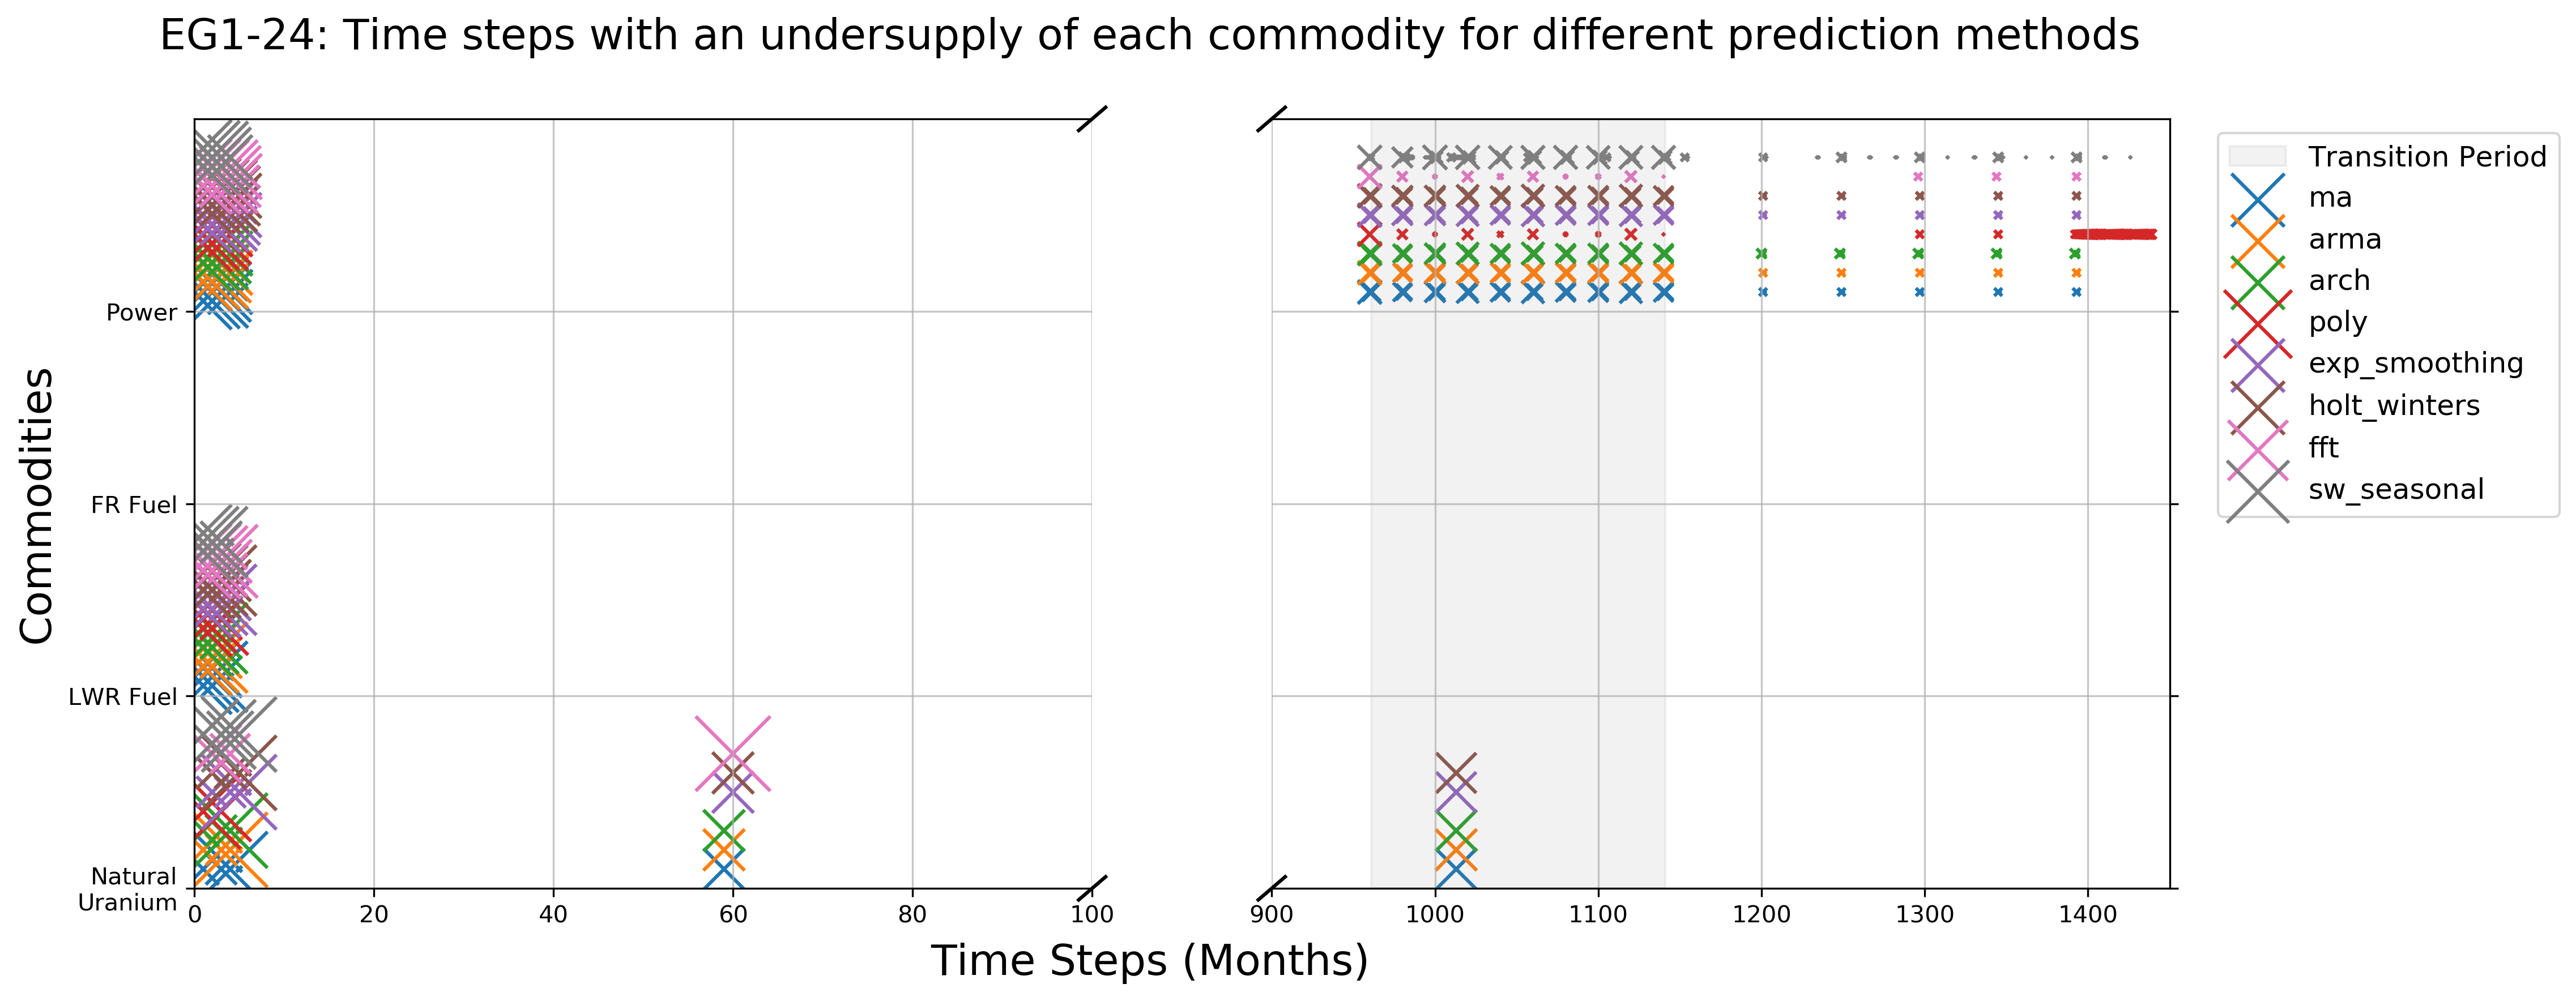
\includegraphics[width=\textwidth]{images/eg24-undersupply.png}
    \end{center}
          \caption{Time dependent undersupply of commodities for different
          prediction methods for the EG01-24 Transition Scenario with Linearly Increasing Power Demand. The
          size of each cross is based on the size of the under capacity.
          Fewer crosses on plot indicates the method is more successful at preventing under capacity
          of each commodity}
  \end{figure}
\end{frame}

\begin{frame}
  \frametitle{Comparison of Prediction Methods}
  \textbf{Main Takeaway}
  \\
  The best performing prediction method for each transition scenario is: 
  \begin{enumerate}
    \item EG01-23 Constant Power Demand: \texttt{poly}
    \item EG01-24 Linearly Increasing Power Demand: \texttt{fft}
    \item EG01-29 Constant Power Demand: \texttt{poly}
    \item EG01-30 Linearly Increasing Power Demand: \texttt{fft}
\end{enumerate}
\end{frame}
